\documentclass{beamer}

\usetheme{AUTheme}
\usefonttheme[onlymath]{serif}

\usepackage{amsmath, latexsym, color, graphicx, amssymb, here}
\usepackage{epsf, epsfig, pifont,tikz}
\usepackage{graphics, calrsfs}
\usepackage{tangocolors}
\usepackage{times}
\usepackage{fancybox,calc}
\usepackage{hyperref}
\usepackage{pgfplots}
\usepackage{verbatim}

\newcommand{\parD}[2]{\frac{\partial #1}{\partial #2}}
\newcommand{\parDD}[2]{\frac{\partial^2 #1}{\partial #2 ^2}}
\newcommand{\laplacian}{\Delta}
\renewcommand{\div}{\nabla\cdot}
\newcommand{\grad}{\nabla}
\newcommand{\divp}{\nabla^\prime\cdot}
\newcommand{\gradp}{\nabla^\prime}
\newcommand{\curl}{\nabla\times}
\newcommand{\cross}{\times}
\renewcommand{\dot}{\cdot}

% define some colors
\definecolor{cBlue}{rgb}{.255,.41,.884} % RoyalBlue of svgnames
\definecolor{cRed}{rgb}{1, 0, 0} % Red of svgnames

%\usecolortheme[named=blue]{structure}
%------------------------------------------------------------Slide 1
\title{Fonts in \LaTeX}
\author{{Kailash Jajam}}
\institute{Dept. of Mechanical Engineering\\ Auburn University, AL}
\date{\today}
%------------------------------------------------------------Slide 1
\begin{document}


\frame{\titlepage}
%\slideCaption{\LaTeX}

%------------------------------------------------------------Slide 2
%\section{Outline}

\begin{frame}[fragile]
\frametitle{Outline:}
\vspace{-0.3cm}

\begin{itemize}
\item Introduction: What is a font?
\item Font file formats
\item How fonts work in general in \LaTeX{}?
\item Font packages in \LaTeX{}
\item \LaTeX{} font attributes
\item Encoding vectors and Mapping schemes
\item Associated \LaTeX{} utilities
\item Specifying font sizes
\item Further reading
\end{itemize}
\end{frame}
%------------------------------------------------------------Slide 2

%------------------------------------------------------------Slide 3
\section{Introduction}

\begin{frame}[fragile]
\frametitle{Introduction}
What is a font?
\begin{itemize}
\item in general terms:\\
      \footnotesize{- collection of glyphs (characters, symbols) of a particular design\\
      - organized into families, series and individual shapes\\
      - can be accessed either by character code or by symbolic names}
\item \normalsize{in technical terms:}\\
      \footnotesize{- different representations depending on the point of view\\
      - \TeX{} typesetter: described by \TeX{} font metrics (TFM)\\
      - DVI driver: virtual fonts (VF), bitmaps fonts (PK), outline fonts (PFA/PFB or TTF)\\
      - PostScript: Type 1 (outlines), Type 3 (anything), Type 42 fonts (embedded TTF)}
\item \normalsize{font information consists of:}\\
      \footnotesize{- metric information (glyph metrics and global parameters)\\
      - glyph shapes (bitmaps and outlines)}
\end{itemize}
\end{frame}
%------------------------------------------------------------Slide 3

%------------------------------------------------------------Slide 4
\section{Font file formats}

\begin{frame}[fragile]
\frametitle{Font file formats}
\begin{itemize}
\item Metafont:\\
      \footnotesize{- TFM, PL: \TeX{} font metrics (binary), property lists (textural)\\
      - VF, VPL: virtual fonts (binary), virtual proerty lists (textural)\\
      - GF, PK: generic fonts, packed fonts (bitmap formats)}
\item \normalsize{PostScript Type 1 outline fonts:}\\
      \footnotesize{- AFM: Adobe font metrics (textural)\\
      - PFM: printer font metrics (binary)\\
      - PFA: printer font ASCII (encoded glyph programs in textural formats)\\
      - PFB: printer font binary (encoded glyph programs in binary formats)}
\item \normalsize{TrueType outline fonts:}\\
      \footnotesize{- TTF: TrueType font(includes both metrics and glyph programs)\\
      - T42: Type 42 font, TrueType font embedded in PostScript wrapper}
\end{itemize}
\end{frame}
%------------------------------------------------------------Slide 4

%------------------------------------------------------------Slide 5
\section{How \LaTeX{} uses fonts}

\begin{frame}[fragile]
\frametitle{How fonts work in general in \LaTeX{}?}
\vspace{-0.3cm}
\begin{figure}[h!]
\centering
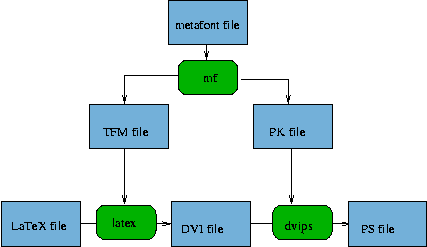
\includegraphics[width=7.5cm]{fig.png}
\vspace{-0.3cm}
\caption{\tiny{\LaTeX{}'s use of metafont fonts}}
\end{figure}
\vspace{-0.75cm}
\begin{itemize}
  \item \scriptsize{TFM and PK files are required.}
  \item \scriptsize{TFM file contains the information about size of each character and how the character will be affected by           neighboring ones in addition to how elastic the space around the character.}
  \item \scriptsize{DVI file contains the coordinates of the characters but not the font shape and the shape of each 
         character can be imparted in two ways:\\
        - as a bitmap: PK files hold bitmaps at set resolutions.\\
        - as a postscrript character.}
\end{itemize}
\end{frame}
%------------------------------------------------------------Slide 5

%------------------------------------------------------------Slide 6
\section{Font packages in \LaTeX{}}

\begin{frame}[fragile]
\frametitle{Font packages in \LaTeX{}}
\vspace{-0.4cm}
\footnotesize{Most \LaTeX{} installations support at least the core set of 13 using the packages below:}\\[5 pt]
\scriptsize{- avant: AvantGrade font as default sans\\
- avantgar: ITC Avant Garde\\
- bookman: Bookman font as default roman\\
- chancery: Zapf Chancery font as default roman\\
- charter: default roman\\
- courier: default ttdefault\\
- helvetic: Helvetica font as default sans\\
- mathpazo: Palatino font as default roman\\
- mathptmx: Times font as default roman\\
- ncntrsbk: NewCenturySchlbk-Roman\\
- newcent: NewCenturySchoolbook font as default Roman\\
- palatcm: Palatino + Computer Modern math\\
- pifont: Pi font support (sepcial characters\\
- utopia: Utopia font as default roman\\
- zapfchan: ITC Zapf Chancery as default roman}\\
\footnotesize{To use (for example) Helvetica, one just adds \tiny{\textbackslash usepackage\{helvet\}}}
\end{frame}
%------------------------------------------------------------Slide 6

%------------------------------------------------------------Slide 7
\section{Font attributes}

\begin{frame}[fragile]
\frametitle{\LaTeX{} font attributes}
\vspace{-0.4cm}
\footnotesize{Every text font in \LaTeX{} has five attributes:}\\

\begin{itemize}
\item \scriptsize{encoding - This specifies the order that characters appear in the font (e.g. whether the 65th character is `A'). The most common value for TeX font encoding is OT1. The other predefined option is T1 (extended \TeX{}). There is also US ASCII (7 bit), ISO Latin-1 (8 bit), Adobe Standard Encoding, etc.}\\
\item \scriptsize{family - The name for a collection of fonts, usually grouped under a common name by the font foundry. For example, `Adobe Times' ptm and Knuth's `Computer Modern Roman' cmr are font families.}\\
\item \scriptsize{series - How heavy or expanded a font is. For example, `medium weight', `narrow' and `bold extended' are all series.}\\
\item \scriptsize{shape - The form of the letters within a font family. For example, `italic', `oblique' and `upright' are all font shapes.}\\
\item \scriptsize{size - The design size of the font, for example `10pt'.}
\end{itemize}
\vspace{-0.3cm}
\scriptsize{The commands to change font attributes are illustrated by the following example:}\\
\tiny{ 
\textbackslash fontencoding\{T1\}\\
\textbackslash fontfamily\{garamond\}\\
\textbackslash fontseries\{m\}\\
\textbackslash fontshape\{it\}\\
\textbackslash fontsize\{12\}\{15\}\\
\textbackslash selectfont\\
}
\scriptsize{This series of commands set the current font to medium weight italic garamond 12pt type with 15pt leading in the T1 encoding scheme, and the} \tiny{\textbackslash selectfont} \scriptsize{command causes LaTeX to look in its mapping scheme for a metric corresponding to these attributes.}
\end{frame}
%------------------------------------------------------------Slide 7

%------------------------------------------------------------Slide 8
%\section{Font attributes}

\begin{frame}[fragile]
\frametitle{Encoding vectors and Mapping schemes}
\vspace{-0.8cm}
\footnotesize{\LaTeX{} typesets use a particular encoding vector and a particular font metric scaled to a particular size depending upon the values of these attributes.}\\

\begin{itemize}
\item \scriptsize{Encoding vector- a set of instructions to LaTeX detailing how particular symbols are to be constructed. For example, the T1 encoding vector file T1enc.def contains the following commands, among many others:}\\[5 pt]
\tiny{ 
  \textbackslash DeclareFontEncoding\{T1\}\{\}\{\}\\
  \textbackslash DeclareTextAccent\{\textbackslash'\}\{T1\}\{1\}\\
  \textbackslash DeclareTextSymbol\{\textbackslash ae\}\{T1\}\{230\}\\
  \textbackslash DeclareTextComposite\{\"\}\{T1\}\{a\}\{228\}}
\item \scriptsize{Mapping schemes - Once a the relevent encoding vector is defined, you may want to set up a scheme which maps font attribute sets to font metrics. For example, the file T1garamond.fd contains the commands}\\[5 pt]
\tiny{
  \textbackslash DeclareFontFamily\{T1\}\{garamond\}\{\}\\
  \textbackslash DeclareFontShape\{T1\}\{garamond\}\{m\}\{n\}\{ \textless-\textgreater garrm \}\{\}\\
  \textbackslash DeclareFontShape\{T1\}\{garamond\}\{m\}\{it\}\{ \textless-\textgreater garit \}\{\}
  }
\end{itemize}
\end{frame}
%------------------------------------------------------------Slide 8

%------------------------------------------------------------Slide 9
\section{\LaTeX{} font utilities}

\begin{frame}[fragile]
\frametitle{Associated \LaTeX{} utilities}
\vspace{-0.3cm}
\footnotesize{\LaTeX{} packages to support new fonts usually contain detailed installation details:}\\
\begin{itemize}
\item \tiny{afm2tfm} - \scriptsize{This will create a TFM files of raw fonts and vpl files of virtual fonts from an AFM file.}
\item \tiny{ttf2tfm} - \scriptsize{TrueType to TFM}
\item \tiny{ttf2afm} - \scriptsize{TrueType to AFM}
\item \tiny{ttf2ptl} - \scriptsize{TrueType to AFM and PFB}
\item \tiny{vptovf} - \scriptsize{From a} \tiny{VPL} \scriptsize{file this creates vf and tfm files for virtual fonts.}
\item \tiny{mf} - \scriptsize{processes a metafont file to produce TFM and PK files.}
\end{itemize}
\end{frame}
%------------------------------------------------------------Slide 9

%------------------------------------------------------------Slide 10
\section{\TeX{} font names}

\begin{frame}[fragile]
\frametitle{\TeX{} font names}
\vspace{-0.3cm}
\footnotesize{In the configuration files the fonts are codenamed. The naming scheme is} \tiny{ FNW\{V\}E\{n\}}\footnotesize{ where:}\\
\begin{itemize}
\item \tiny{F} - \scriptsize{is a one-letter abbreviation for the foundry (m = monotype, p = adobe, b = bitstream, f = free)}
\item \tiny{N} - \scriptsize{is a two letter abbreviation for the font name (for example, ag = "avant garde")}
\item \tiny{W} - \scriptsize{is the font weight (r = regular, b = bold, l = light d = demibold)}
\item \tiny{V} - \scriptsize{is an optional slope variant (i = italic , o = oblique)}
\item \tiny{E} - \scriptsize{is an abbreviation for the encoding (almost always 8a which is adobe standard encoding).}
\item \tiny{N} - \scriptsize{ is an optional width variant (n = narrow)}
\end{itemize}
\footnotesize{For example, the font Adobe Garamond demibold is}\tiny{ pgad8a.}  
\end{frame}
%------------------------------------------------------------Slide 10

%------------------------------------------------------------Slide 11
%\section{Useful example}

\begin{frame}[fragile]
\frametitle{Useful example}
\vspace{-0.7cm}
\footnotesize{In order to select another than the default typeface in LaTeX environment, it is necessary to include some commands in the preamble of the document.}\\[5 pt]
\footnotesize{Consider the following example:}\\[5 pt]
\tiny{\textbackslash usepackage[T1]\{fontenc\}}\\[5 pt]
\tiny{\textbackslash usepackage[light,math]\{iwona\}}\\[15 pt]
\tiny{\textbackslash documentclass\{book\}}\\[5 pt]
\tiny{\textbackslash newcommand\textbackslash blah\{blah blah blah\}}\\[5 pt]
\tiny{\textbackslash blah \textbackslash blah }\\[5 pt]
\tiny{\textbackslash renewcommand*\textbackslash rmdefault\{ppl\}\textbackslash normalfont\textbackslash upshape}\\[5 pt]
\tiny{\textbackslash blah \textbackslash blah }\\[5 pt]
\tiny{\textbackslash renewcommand*\textbackslash rmdefault\{iwona\}\textbackslash normalfont\textbackslash upshape}\\[5 pt]
\tiny{\textbackslash blah \textbackslash blah }\\
\tiny{\textbackslash end\{document\}} 
\end{frame}
%------------------------------------------------------------Slide 11


%------------------------------------------------------------Slide 12
\section{Furhter reading}

\begin{frame}[fragile]
\frametitle{Furhter reading}
\vspace{-0.3cm}
\normalsize{Detailed description can be found at:}\\

\begin{itemize}
\item \footnotesize{http://www.cl.cam.ac.uk/\~{}rf10/pstex/latexcommands.htm}
\item \footnotesize{http://www-h.eng.cam.ac.uk/help/tpl/textprocessing/fonts.html}
\item \footnotesize{ftp://tug.ctan.org/tex-archive/fonts/utilities/fontinst/doc/talks/et99-font-tutorial.pdf}
\end{itemize}
\end{frame}
%------------------------------------------------------------Slide 12


%------------------------------------------------------------Slide 13
\begin{frame}[fragile]
\frametitle{}
\centering \Huge{Thank You}
\end{frame}
%------------------------------------------------------------Slide 13

\end{document}